
Learning from interactions with users is ubiquitous in modern customer-facing systems, from product recommendations to web search to content selection to fine-tuning user interfaces. Many systems purposefully implement \emph{exploration}: making potentially suboptimal choices for the sake of acquiring new information.
Online platforms routinely deploy A/B tests, and are increasingly adopting  more sophisticated exploration methodologies based on \emph{multi-armed bandits}, a well-known framework for exploration and making decisions under uncertainty. 


%~\cite{KohaviAB-2015,KohaviLSH09}

In this paper, we initiate a study of the interplay between \exploration and \competition. Systems that engage in exploration typically need to compete against one another; most importantly, they compete for users. This creates a tension:
%between \exploration and \competition. 
while exploration may be essential for improving the service tomorrow, it may degrade quality and make users leave \emph{today}, in which case there will be less users to learn from. This may further degrade the platform's performance relative to competitors who keep learning and improving from \emph{their} users, and so forth. Taken to the extreme, such dynamics may create a ``death spiral" effect when the vast majority of customers eventually switch to competitors. Users therefore serve three distinct roles: they are customers that generate revenue, they are sources of data for learning, and they are self-interested agents who choose among the competing systems.

\ascomment{stopped here.}

The main high-level question that we focus on in this paper is whether competition between systems incentives the adoption of better exploration algorithms. This translates into a number of more concrete questions. While it is commonly assumed that ``better" technology always helps, is this so for our setting? Does increasing competition lead to higher consumer welfare? To what extent is there a ``data feedback loop" where one firm having more data leads to that firm attracting more users which leads to that firm having more data, etc.?\footnote{This is a fundamental question which is part of a larger policy discussion around whether data can serve as an indirect network effect and lead to similar ``market tipping" results as is standard in the literature on competition in markets with network effects (see \cite{jullien2019economics} for a policy oriented discussion of this).}

% the extent to which the game between the two principals is competitive
% degree of innovation that these models incentivize.
% the extent to which agents make rational decisions


%\subsection{Our model}
%\label{sec:intro-model}

\xhdr{Our model.} We investigate these questions with a stylized duopoly model where two firms commit to exploration strategies and compete for a stream of consumers. We define a game in which two firms (\emph{principals}) simultaneously engage in exploration and compete for users (\emph{agents}). These two processes are interlinked, as exploration decisions are experienced by users and informed by their feedback. We need to specify several conceptual pieces: how the principals and agents interact, what is the machine learning problem faced by each principal, and what is the information structure. Each piece can get rather complicated in isolation, let alone jointly, so we strive for simplicity. Thus, the basic model is as follows:

\begin{itemize}

\item A new agent arrives in each round $t=1,2, \ldots$, and chooses among the two principals. The principal chooses an action (\eg a list of web search results to show to the agent), the user experiences this action, and reports a reward. All agents have the same ``decision rule" for choosing among the principals given the available information.

\item Each principal faces a very basic and well-studied version of the multi-armed bandit problem: for each arriving agent, it chooses from a fixed set of actions  (a.k.a. \emph{arms}) and receives a reward drawn independently from a fixed distribution specific to this action.

\item Principals simultaneously announce their learning algorithms before round $1$, and cannot change them afterwards. There is a common Bayesian prior on the rewards (but the realized reward distributions are not observed by the principals or the agents).  Each principal only observes agents that chose him. We consider two variants of the baseline model and the information set for the agent differs between the two:
\begin{enumerate}
\item In the \textit{expectation choice variant}, agents do not receive any other information and choose between the principals using their knowledge of $t$ and the principals' algorithms.
\item In the \textit{reputation choice variant}, agents have access to a reputation score for each principal, which is a sliding window average of the rewards experienced by previous agents that have visited this principal.
\end{enumerate}
\end{itemize}

\xhdr{Main Findings.}
We find that competition induces firms to commit to a greedy (myopic) algorithm in equilibrium that does no purposeful exploration. This leads to low consumer welfare since the greedy algorithm is known to be dramatically bad in many important cases of multi-armed bandits. The primary mechanism that generates this stark result is that consumers need to be incentivized to select a firm over its competitors, leading a firm that engages in exploration to be starved of consumers before it makes enough progress on its learning problem. In order to incentivize ``better" exploration strategies in equilibrium, the key intuition is that the firm needs to have some ``free" consumers that visit them without the firm having to incentivize them to do so. This allows the firm to eventually overcome the initial losses in consumer perception from exploration. We explore two economic mechanisms that can generate such an effect.

The first is the presence of users who randomly choose between the firms which gives each firm a constant stream of ``free" users and thus ensures it never gets fully starved. We find that, even when there is a small fraction of such consumers, better algorithms help in a big way: a sufficiently better algorithm is guaranteed to win all non-random agents after an initial learning phase.\footnote{While the precise notion of ``sufficiently better algorithm" is rather subtle, we note that commonly known ``smart" bandit algorithms typically defeat the commonly known ``naive" ones, and the latter typically defeat the greedy algorithm. However, there is a substantial caveat: one can defeat any algorithm by interleaving it with the greedy algorithm. This has two undesirable corollaries: a better algorithm may sometimes lose, and a pure Nash equilibrium typically does not exist.} However, while this holds asymptotically, our numerical experiments show that this requires either unreasonably large time scales or a large fraction of such users.

The second is that if one firm has a first-mover advantage then this firm gets free users before the other firm enters into the market. We show that if this incumbency period is sufficiently long, then it allows the firm to make sufficient progress on its learning problem and incentivizes it to commit to better algorithms. While this leads to the incumbent getting almost all of the market, it leads to higher consumer welfare than under competition when the firms enter at the same time.

\xhdr{\underline{Additional Findings}}

\xhdr{Reputation and Data Advantage}: In the reputation choice variant we investigate the first-mover advantage phenomenon in more detail. Being first in the market gives the incumbent free data to learn from (a ``data advantage") as well as a more definite, and possibly better reputation compared to an entrant (a ``reputation advantage"). We run additional experiments so as to isolate and compare these two effects. We find that either effect alone leads to a significant advantage under competition. The data advantage is larger than reputation advantage when the incumbent commits to a more advanced bandit algorithm. This result shows that even a small amount ``data advantage" gets amplified under competition, causing a large difference in eventual market shares.

\xhdr{Noise in consumer choice}: We further relax the decision rule of the agents so that the probability of choosing a given firm varies smoothly as a function of the difference between  principals' expected rewards. For this decision rule, the ``better algorithm wins" result holds under much weaker assumptions on what constitutes a better algorithm. This is the most technical result of the paper. The competition in this setting is necessarily much more relaxed: typically, both principals attract approximately half of the agents as time goes by (but a better algorithm may attract slightly more).

\xhdr{Predicting Outcomes in Competition} We also investigate how algorithms' performance ``in isolation" (without competition) is predictive of the outcomes under competition in the reputation choice variant. We find that mean reputation -- arguably, the most natural performance measure ``in isolation" -- is sometimes not a good predictor. We suggest a more refined performance measure, based on a comparison between the reputation of the two firms, and use it to explain some of the competition outcomes.
\textbf{Add some discussion about comparison with ``better" algorithms in analytical part}

\OMIT{All results extend to a much more general version of the multi-armed bandit problem in which the principal may observe additional feedback before and/or after each decision, as long as the feedback distribution does not change over time. In most results, principal's utility may depend on both the market share and agents' rewards.
}

\begin{figure}
\begin{center}
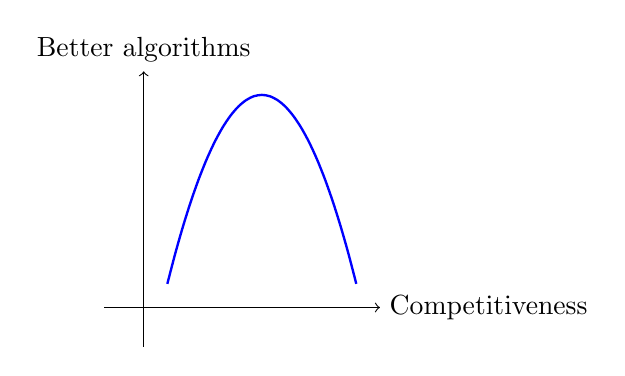
\begin{tikzpicture}
      \draw[->] (-.5,0) -- (3,0) node[right] {Competitiveness};
      \draw[->] (0,-.5) -- (0,3) node[above] {Better algorithms};
      \draw[scale=0.6,domain=0.5:4.5,smooth,variable=\x,blue, line width=0.3mm] plot ({\x},{4.5 - (\x - 2.5)^2});
      % \draw[scale=0.5,domain=-3:3,smooth,variable=\y,red]  plot ({\y*\y},{\y});
 \end{tikzpicture}

\caption{Inverted-U relationship between competitiveness and algorithms.}
\label{fig:inverted-U}
\end{center}
\end{figure}
\xhdr{Economic interpretation.} Our model speaks to two distinct strands of the economics literature.

The first is the literature that studies the relationship between competition and innovation where, in our context,  the choice between different algorithms is interpreted as firms determining whether to invest in a ``better" technology as the degree of competition varies.\footnote{The choice of algorithms has a clear analogue to ``innovation" in our context as the literature on multi-armed bandits has identified distinct ``classes" of algorithms according to asymptotic regret bounds. Thus, choosing algorithms in ``better" classes corresponds with innovation on the part of the firm in our interpretation of the model. It is not salient whether similar ideas and/or technologies already exist outside the firm. It is worth noting that the adoption of exploration algorithms tends to require substantial R\&D effort in practice, even if the algorithms themselves are well-known in the research literature; see \citet{MWT-WhitePaper-2016} for an example of such R\&D effort.} A classic result in this literature is that there is an inverted-U relationship between the severity of competition among firms and the quality of technologies that they adopt is a familiar theme in the economics literature \citep[\eg][]{Aghion-QJE05,Vives-08}.

We find it illuminating to frame our contributions in a similar manner, as illustrated in \reffig{fig:inverted-U}. In our model we consider varying the intensity of competition as varying the degree to which a firm needs to incentivize users to visit them. Competition is less intense when there are more ``random" users or one firm has a sufficiently long first-mover advantage. The inverted-U relationship in our model arise for a fundamentally different reason, compared to the existing literature on ``competition vs. innovation.'' In the literature, better technology always helps in a competitive environment, other things being equal. Thus, the trade-off is between the costs of improving the technology and the benefits that the improved technology provides in the competition. Meanwhile, we find that a better exploration algorithm may sometimes perform much worse under competition, even in the absence of R\&D costs. This stems from the nature of exploration technologies in online markets which rely on learning from interactions with users. This leads to an implicit cost from exploration in the form of a reduced rate of users that a firm attracts and can learn from.

Interestingly, the economic mechanism in our model for incentivizing firms to engage in R\&D has a qualitative similarity to the role that patents play in incentivizing innovation in standard R\&D models. In these models, patents temporarily relax competition for the innovating firm by giving them exclusive access to their innovation for a limited period of time in order to incentivize them to invest in the better technology. In our model, temporarily relaxing competition in the form of giving firms free periods to learn incentivizes the firm to invest in the better technology.

The second is the nascent literature which studies the economics of data and how data can serve as a barrier to entry in the digital economy \cite{de2020data, hagiu2020data}. Our model directly speaks to this literature as we endogenize data-driven network effects by explicitly considering a model where firms are simultaneously solving a machine learning problem while competing against each other for users. The results of our model point to the fact that competition dynamics -- that firms compete as they learn over time and that this competition endogenously determines the data observed by firms -- are pertinent to understanding whether or not data can serve as a barrier to entry. Indeed, our results are similar to the market tipping results in the literature on indirect network effects and show a channel through which differences in data ownership can result in market tipping. However, it is important to note that the channel through which this arises in our model is not simply from differences in the quantity of data possessed by the firms, but also from the quality of the data.

\xhdr{Discussion}
We consider two separate variants of the model in order to provide a more thorough investigation of the tension between exploration and competition. The expectation choice model is tractable enough to allow us to obtain theoretical results with ``asymptotic" flavor. However, for the sake of analytical tractability, we make the unrealistic simplification that users do not observe any signals about firms' ongoing performance and it is difficult to analyze important economic mechanisms such as asymmetries in the timing of entry.

The reputation choice model relaxes this simplification and accounts for competition in a more direct way as well as allows us to explore other relevant economic mechanisms in understanding the tension between exploration and competition. However, it now becomes considerably harder to analyze analytically. This is for several reasons: intricate feedback loop from performance to reputations to users to performance;
%
mean reputation, most connected to our intuition, is sometimes a bad predictor in competition (see Sections~\ref{sec:isolation} and~\ref{sec:revisited});
%
mathematical tools from regret-minimization would only produce ``asymptotic" results, which do not seem to suffice. We therefore analyze our model using numerical simulation, which has several benefits. It allows us to analyze our model from a ``non-asymptotic" perspective, looking for substantial effects within relevant time scales. Indeed, we start our investigation by determining what time scales are relevant in the context of this variant of the model. Further, it allows us to investigate important economic mechanisms that arise in environments where exploration and competition tensions are at play, such as the effect of incumbency, increasing the number of firms, and the extent to which data can serve as a barrier to entry.

\xhdr{Map of the paper.}
We survey related work (Section~\ref{sec:related-work}), lay out the model and preliminaries (Section~\ref{sec:model}). We start by analyzing the expectation choice model analytically. In Sections ~\ref{sec:rational},~\ref{sec:random}, and ~\ref{sec:soft} we analyze the expectation choice variant and characterize the equilibrium behavior under three different agent decision rules. Then, we turn to analyze the reputation choice variant of the model with details of the analysis described in Section ~\ref{sec:sim_details}. Sections ~\ref{sec:isolation} and ~\ref{sec:revisited} overview results from running different bandit algorithms in isolation (i.e. without competition). Sections ~\ref{sec:competition} and ~\ref{sec:barriers} overview the results of the reputation choice variant. Section ~\ref{sec:non_greedy} presents results of varying the consumer choice rule in the reputation choice variant. Section ~\ref{sec:conclusion} concludes.


%%% Local Variables:
%%% mode: latex
%%% TeX-master: "main"
%%% End:
